\documentclass[11pt,a4paper]{article}

\usepackage[margin=2.3cm]{geometry}
\usepackage[T1]{fontenc}
\usepackage[utf8]{inputenc}
\usepackage{lmodern}
\usepackage{textcomp}
\usepackage{microtype}
\usepackage{amsmath}
\usepackage{booktabs}
\usepackage{graphicx}
\usepackage{hyperref}
\usepackage{xcolor}
\usepackage{listings}
\usepackage{tikz}
\usetikzlibrary{arrows.meta,positioning,shapes.geometric,calc,fit,backgrounds}

\hypersetup{
    colorlinks=true,
    linkcolor=black!70,
    urlcolor=blue!60!black,
}

\lstset{
    basicstyle=\ttfamily\footnotesize,
    columns=fullflexible,
    keepspaces=true,
    breaklines=true,
    showstringspaces=false,
    frame=single,
    framesep=3pt,
    xleftmargin=6pt,
}

\title{\vspace{-1cm}Assignment 1: Text Processing Fundamentals using MapReduce\\
       \large Chi-Square Term Selection over 22 Amazon Review Categories}
\author{
Group 48 -- Data-Intensive Computing, TU Wien, SS~2026\\[2pt]
\small
Aaradhaya Arora (12534787) \quad
Ekaterina Dobrynina (12332276) \quad
Gopinath Hariharasudhan (52202173) \\[1pt]
\small
Serhii Slutu (12537831) \quad
Sofia Zubkova (12534780)
}
\date{\today}

\begin{document}
\maketitle

\vspace{-0.4cm}

\noindent\textbf{AI disclosure.}
We used Anthropic's Claude Opus 4.7 as a support tool while working on this
assignment. Its use was limited to text polishing (grammar, wording) and to
debugging help when we were stuck. The pipeline design, the choice of
\texttt{<key,value>} pairs, the chi-square derivation and all
implementation decisions were made by us; the model did not generate ideas
or solutions, it was used purely as assistance.

\vspace{0.2cm}

%==============================================================
\section{Introduction}
%==============================================================

The goal of this assignment is to pick, for each of the 22 Amazon review
categories, the terms that are most useful for telling one category apart
from the others -- a typical feature selection step before any real text
classifier is trained. We use the chi-square test for that, because it
only needs document-frequency counts and fits MapReduce nicely.

The dataset is big enough that we cannot simply load it into memory: the
course provides a small development set (\texttt{reviews\_devset.json},
about 78\,800 reviews) and a full 56\,GB version on HDFS. We developed
and tested everything on the development set and wrote the code so that
running it on the full corpus is just a matter of changing the input
path.

In the rest of this report we describe the structure of the pipeline,
what each mapper and reducer actually does (including the
\texttt{<key,value>} pairs that flow between them) and what the output
on the development set looks like.

%==============================================================
\section{Problem Overview}
%==============================================================

\paragraph{Input.}  Each line of the input file is a JSON document. Out of all
the fields we only look at two: \texttt{reviewText} (the text to process)
and \texttt{category} (the class label).

\paragraph{Pre-processing.}  Before counting anything we have to clean up
the text. The steps are the ones described in the assignment:

\begin{itemize}
  \item lowercase the review text,
  \item split on whitespace, tabs, digits and the characters
    %
    \begin{center}\footnotesize
    \verb|( ) [ ] { } . ! ? , ; : + = - _ " ' ` ~ # @ & * % $ \ /|
    \end{center}
    %
    plus \texttt{\texteuro} and \texttt{\S},
  \item drop tokens that are in \texttt{stopwords.txt} or that have
    length 1.
\end{itemize}

Because chi-square cares about \emph{how many documents} contain a term
in a given category (not how many times it occurs), we also de-duplicate
the tokens of a review before counting them. So from every review we
keep a \emph{set} of unigrams.

\paragraph{Chi-square.}  For a term $t$ and a category $c$ we build the usual
$2\times 2$ contingency table:
\[
\begin{array}{c|cc}
               & t\in d      & t\notin d    \\ \hline
d\in c         & A           & C            \\
d\notin c      & B           & D            \\
\end{array}
\qquad N=A+B+C+D.
\]
Here $A$ is the number of documents of category $c$ that contain $t$.
If we also know $n_c$ (the size of category $c$) and $f_t = A+B$ (how
many documents in total contain $t$), we can fill in the other cells
directly:
\[
B = f_t - A,\qquad C = n_c - A,\qquad D = N - n_c - B.
\]
With the standard simplified formula,
\begin{equation}
    \chi^{2}(t,c) \;=\; \frac{N\,(AD-BC)^{2}}{(A+B)(A+C)(B+D)(C+D)},
    \label{eq:chi2}
\end{equation}
we can compute $\chi^2$ from just four numbers: $A$, $f_t$, $n_c$ and
$N$. This is convenient, because the first MapReduce job is going to
produce exactly those.

\paragraph{Output.}  What we have to produce is one text file,
\texttt{output.txt}, with:

\begin{itemize}
    \item one line per category, sorted alphabetically, in the format
      \mbox{\small\texttt{<category>\ t$_1$:$\chi^2_1$\ \ldots\ t$_{75}$:$\chi^2_{75}$}};
    \item one final line with the merged dictionary, i.e.\ all terms
      that appear in any of the 22 top-75 lists, sorted alphabetically
      and space-separated.
\end{itemize}

%==============================================================
\section{Methodology and Approach}
%==============================================================

\subsection{Pipeline overview}
\label{sec:pipeline}

We split the work into two MapReduce jobs. The first one counts; the
second one computes chi-square, picks the top-75 per category and
builds the merged dictionary. A tiny text file (\texttt{meta.tsv},
under one kilobyte) is produced by the driver between the two jobs and
carries the category sizes $n_c$ and the global count $N$ to the
second job.

Figure~\ref{fig:pipeline} shows the whole pipeline with the
\texttt{<key,value>} pair on every arrow, which is the design contract
we tried to keep as explicit as possible.

\begin{figure}[p]
    \centering
    \resizebox{!}{0.84\textheight}{% Standalone TikZ pipeline figure -- included from report.tex
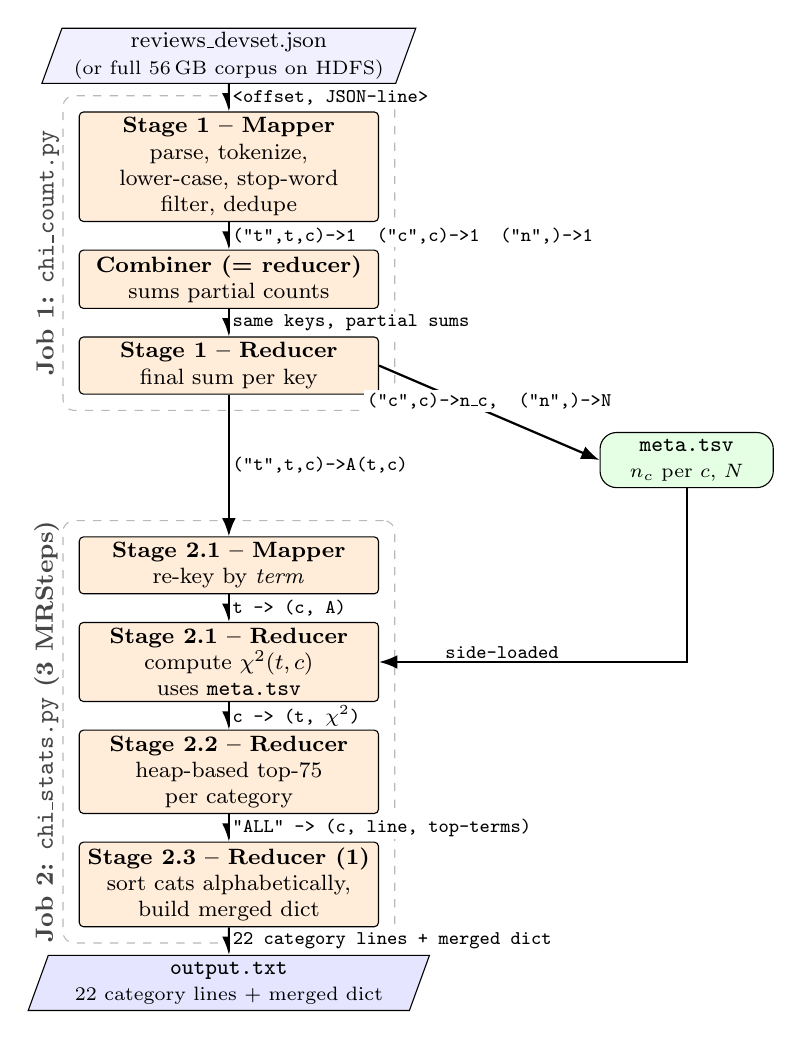
\begin{tikzpicture}[
    font=\footnotesize,
    node distance = 3.5mm and 8mm,
    every node/.style = {align=center},
    data/.style   = {draw, trapezium, trapezium left angle=70, trapezium right angle=110,
                     minimum width=26mm, minimum height=7mm, fill=blue!6,
                     inner sep=1pt},
    stage/.style  = {draw, rectangle, rounded corners=1.5pt, minimum width=38mm,
                     minimum height=7mm, fill=orange!15, line width=0.4pt,
                     inner sep=2pt},
    meta/.style   = {draw, rectangle, rounded corners=6pt, fill=green!10,
                     minimum width=22mm, minimum height=7mm, inner sep=2pt},
    arr/.style    = {-Latex, thick},
    kv/.style     = {font=\scriptsize\ttfamily, fill=white, inner sep=1pt},
    group/.style  = {draw=gray!55, dashed, rounded corners, inner sep=2mm},
    grouplabel/.style = {font=\small\bfseries, rotate=90, inner sep=1pt,
                         text=gray!55!black},
]

% ---------------- Input ----------------
\node[data] (in) {reviews\_devset.json\\\scriptsize (or full 56\,GB corpus on HDFS)};

% ---------------- Stage 1 ----------------
\node[stage, below=of in] (s1map)  {\textbf{Stage 1 -- Mapper}\\parse, tokenize,\\lower-case, stop-word\\filter, dedupe};
\node[stage, below=of s1map] (s1comb) {\textbf{Combiner (= reducer)}\\sums partial counts};
\node[stage, below=of s1comb] (s1red) {\textbf{Stage 1 -- Reducer}\\final sum per key};

\begin{pgfonlayer}{background}
\node[group, fit=(s1map)(s1comb)(s1red)] (s1) {};
\node[grouplabel, anchor=south] at (s1.west) {Job~1: \texttt{chi\_count.py}};
\end{pgfonlayer}

% ---------------- Meta side-file (placed between the two groups) ----------------
\node[meta, right=28mm of s1red, yshift=-12mm] (meta) {\texttt{meta.tsv}\\\scriptsize $n_c$ per $c$,\ $N$};

% ---------------- Stage 2 ----------------
\node[stage, below=18mm of s1red] (s2m1) {\textbf{Stage 2.1 -- Mapper}\\re-key by \emph{term}};
\node[stage, below=of s2m1]      (s2r1) {\textbf{Stage 2.1 -- Reducer}\\compute $\chi^2(t,c)$\\uses \texttt{meta.tsv}};
\node[stage, below=of s2r1]      (s2r2) {\textbf{Stage 2.2 -- Reducer}\\heap-based top-75\\per category};
\node[stage, below=of s2r2]      (s2r3) {\textbf{Stage 2.3 -- Reducer (1)}\\sort cats alphabetically,\\build merged dict};

\begin{pgfonlayer}{background}
\node[group, fit=(s2m1)(s2r1)(s2r2)(s2r3)] (s2) {};
\node[grouplabel, anchor=south] at (s2.west) {Job~2: \texttt{chi\_stats.py} (3 MRSteps)};
\end{pgfonlayer}

% ---------------- Output ----------------
\node[data, below=of s2r3, fill=blue!10] (out) {\texttt{output.txt}\\\scriptsize 22 category lines + merged dict};

% ---------------- Arrows with <k,v> labels ----------------
\draw[arr] (in) -- (s1map)
    node[kv, midway, right]{<offset, JSON-line>};

\draw[arr] (s1map) -- (s1comb)
    node[kv, midway, right]{("t",t,c)->1 \ ("c",c)->1 \ ("n",)->1};

\draw[arr] (s1comb) -- (s1red)
    node[kv, midway, right]{same keys, partial sums};

\draw[arr] (s1red.east) -- (meta.west)
    node[kv, midway, above]{("c",c)->n\_c,\ \ ("n",)->N};

\draw[arr] (s1red) -- (s2m1)
    node[kv, midway, right]{("t",t,c)->A(t,c)};

\draw[arr] (s2m1) -- (s2r1)
    node[kv, midway, right]{t -> (c, A)};

\draw[arr] (meta.south) |- (s2r1.east)
    node[kv, pos=0.8, above]{side-loaded};

\draw[arr] (s2r1) -- (s2r2)
    node[kv, midway, right]{c -> (t, $\chi^2$)};

\draw[arr] (s2r2) -- (s2r3)
    node[kv, midway, right]{"ALL" -> (c, line, top-terms)};

\draw[arr] (s2r3) -- (out)
    node[kv, midway, right]{22 category lines + merged dict};

\end{tikzpicture}
}
    \caption{End-to-end chi-square pipeline. Every arrow is labelled with
             the \texttt{<key,value>} pair that flows through it.
             Orange rectangles are MapReduce tasks, the blue
             parallelograms are data sets on disk, and the green rounded
             box is the small meta file that the driver passes from the
             first job to the second.}
    \label{fig:pipeline}
\end{figure}

\subsection{Stage~1 -- counting}

The first job (\texttt{chi\_count.py}) reads the JSON review lines and
emits three kinds of records:

\begin{center}\small
\begin{tabular}{@{}lll@{}}
    \toprule
    Record                           & Meaning                                  & Useful for \\
    \midrule
    \texttt{(("t",\,t,\,c),\,1)}     & document contains term $t$ in category $c$ & $A(t,c)$ \\
    \texttt{(("c",\,c),\,1)}         & document belongs to category $c$          & $n_c$     \\
    \texttt{(("n",),\,1)}            & one more document seen                    & $N$       \\
    \bottomrule
\end{tabular}
\end{center}

In the mapper we keep per-task Python dictionaries
(\texttt{\_buf\_tc}, \texttt{\_buf\_c} and a counter \texttt{\_buf\_n})
and only emit the records in \texttt{mapper\_final()}. This is the
in-mapper combining pattern and it cuts the amount of data going into
the shuffle a lot, because a term that appears in many reviews of the
same split is aggregated locally first. A normal combiner with the
same logic as the reducer sits on top of it. The reducer simply sums
the partial counts for each key.

\subsection{Between the two jobs -- \texttt{meta.tsv}}

The driver (\texttt{run.sh} on the cluster, \texttt{run\_local.py} for
local testing) reads the Stage-1 output once, keeps only the
\texttt{"c"} and \texttt{"n"} records and writes a tiny TSV file:

\begin{lstlisting}[caption={\texttt{meta.tsv} (excerpt)}]
n	78829
c	Apps_for_Android	2638
c	Automotive	1374
...
\end{lstlisting}

The term-level records stay on HDFS; only this small file is shipped
to the Stage-2 tasks via mrjob's \texttt{--file} mechanism. We chose
this over the two obvious alternatives -- either replicating $n_c$ and
$N$ on every term record (which would blow up the shuffle) or sending
everything through a single reducer (which would kill parallelism).

\subsection{Stage~2 -- chi-square, top-75 and merged dictionary}

The second job (\texttt{chi\_stats.py}) has three MRSteps:

\begin{enumerate}
    \item \textbf{Regroup by term.} The mapper re-emits each count as
          \texttt{(term, (cat, A))}. The \texttt{"c"} / \texttt{"n"}
          records from Stage 1 are simply ignored here, because that
          information is already in \texttt{meta.tsv} (loaded in
          \texttt{mapper\_init} / \texttt{reducer\_init}). The reducer
          then sees all \texttt{(cat, A)} pairs for a single term in
          one go, which is exactly what we need: we sum them to get
          $f_t$, look up $n_c$ and $N$ in the meta file, derive
          $B$, $C$, $D$ and emit \texttt{(cat, (term, $\chi^2$))}
          using Eq.~\eqref{eq:chi2}. If the denominator is zero (this
          happens only when a term appears exclusively in one
          category) we just skip that pair.
    \item \textbf{Top-75 per category.} The second reducer receives
          all \texttt{(term, $\chi^2$)} pairs of a given category and
          keeps only the 75 best using a bounded min-heap. We emit
          the whole formatted line for the category as one record.
    \item \textbf{Final assembly.} The last step runs with a single
          reducer (forced via \texttt{mapreduce.job.reduces=1}). It
          collects the 22 category lines, sorts them alphabetically,
          prints them, and then prints the merged dictionary. At that
          point the data is tiny -- 22 short lines -- so a single
          reducer is absolutely fine.
\end{enumerate}

\subsection{Design choices and why we made them}

\begin{itemize}
    \item \textbf{Document frequency, not raw frequency.} Deduplicating
          the tokens of each review keeps the $\chi^2$ formula correct
          and also keeps the intermediate key space small.
    \item \textbf{In-mapper combining + combiner.} Together they greatly
          reduce the amount of data that actually goes through the
          shuffle, which is usually the slowest part of a MapReduce job.
    \item \textbf{Meta broadcast via a small side file.} This keeps the
          reducer parallelism intact while still giving every reducer
          access to the global totals it needs.
    \item \textbf{Heap for top-$K$.} $O(V_c \log K)$ per category is
          simpler and faster than sorting and then slicing.
    \item \textbf{Single reducer only at the very end.} We only force
          the sequential bottleneck where the amount of data is
          already tiny.
    \item \textbf{Parameterised input path.} Both drivers take the
          input path as their first argument, so switching from the
          dev set to the full 56\,GB corpus is a one-liner.
\end{itemize}

\subsection{Results on the development set}

We tested the whole pipeline on \texttt{reviews\_devset.json}
(78\,829 reviews, 22 categories). End-to-end it runs in about 20
seconds on a normal laptop using mrjob's inline runner, which is
what we used during development. The resulting \texttt{output.txt}
has exactly the expected shape: 22 category lines of 75 tokens each,
plus one final line with the merged dictionary (1\,463 unique terms
in our case).

The terms that come out on top look sensible for each category, for
instance \textit{music} for \textsc{CDs\_and\_Vinyl}
($\chi^2\!\approx\!13\,083$), \textit{dvd} for
\textsc{Movies\_and\_TV} (${\approx}8\,747$), \textit{reading} for
\textsc{Book} (${\approx}6\,185$), \textit{iphone} for
\textsc{Cell\_Phones\_and\_Accessorie} (${\approx}4\,184$),
\textit{diaper} for \textsc{Baby} (${\approx}2\,430$), and
\textit{cat} for \textsc{Pet\_Supplie} (${\approx}4\,345$). That
matches what we expected from the category names and gave us
confidence that the implementation is doing the right thing.

%==============================================================
\section{Conclusions}
%==============================================================

We built a two-job MapReduce pipeline that turns the Amazon review
corpus into a small, chi-square based vocabulary. Stage 1 handles the
heavy counting, Stage 2 does the statistics and the top-$K$ selection,
and a tiny meta file in between carries the global totals so that
Stage 2 can stay parallel. On the development set the whole thing
runs in about 20 seconds and produces exactly the output format
requested by the assignment. The same code runs on the cluster
without modification -- only the input path changes -- which is what
makes the transition to the full 56\,GB dataset painless for the
final evaluation.

\end{document}
